\section{Приложения $n$-кратного интеграла.}
Рассмотрим некоторые геометрические и механические приложения интегралов ФНП,
а также вычисление интеграла Эйлера-Пуассона.

\subsection{Основные геометрические приложения $n$-кратных
интегралов.}
Основанные приложения $n$-кратного интеграла основаны на использовании формулы:
\begin{equation}
	\label{eq:lecture7-1}
	\mes H = \int\limits_Hdx = \underset{H}{\int \ldots \int}dx_1 \ldots dx_n,
\end{equation}
где $H$ - некоторое измеримое множество в $\R{n}$. В дальнейшем ограничимся
использованием \eqref{eq:lecture7-1} для вычисления площадей квадрируемых плоских
фигур, а также площадей поверхностей и кубируемых тел в $\R{3}$.
\begin{itemize}
  \item $n = 2$. Для площади $S$ квадрируемой плоской фигуры $D \subset \R{2}$ в ПДСК
	$Oxy$ в силу \eqref{eq:lecture7-1}:
	\begin{equation}
		\label{eq:lecture7-2}
		S = \text{пл. } D = \iint\limits_Ddxdy.
	\end{equation}
	В случае, когда $D \subset \R{2}$ - криволинейная трапеция:
	\begin{equation}
		\label{eq:lecture7-3}
		D = \defineset{(x, y) \in \R{2}}{c(x) \leqslant y \leqslant d(x),
		a \leqslant x \leqslant b},
	\end{equation}
	где $c(x)$ и $d(x)$ непрерывны на $\interval[{a; b}]$. Из \eqref{eq:lecture7-2}
	для \eqref{eq:lecture7-3} после перехода к повторным интегралам имеем:
	\begin{equation}
		\label{eq:lecture7-4}
		S = \int\limits_a^bdx\int\limits_{c(x)}^{d(x)}dy = \int\limits_a^b(d(x) - c(x))dx.
	\end{equation}
	Если заранее неизвестно, график какой из кривых ($y = c(x)$ или $y = d(x)$)
	расположен выше, то формула \eqref{eq:lecture7-4} принимает вид хорошо известной из приложений ОИ формулы:
	\begin{equation}
		\label{eq:lecture7-5}
		S = \text{ площадь} D = \int\limits_a^b\abs{c(x) - d(x)}dx.
	\end{equation}
	В связи с этим, использование указанного метода вычисления {ничего нового}
	в сравнении с ОИ не даёт. На практике более удобным способом вычисления
	площади с помощью 2И является замена переменных в 2И.

	Если имеется диффеоморфизм
	\begin{equation*}
		\begin{cases}
			x = x(u, v), \\
			y = y(u, v),
		\end{cases}
        \text{ где }  (u, v) \in G, (x, y) \in D,
	\end{equation*}
	плоских квадрируемых фигур $G \subset \R{2}$ и $D \subset \R{2}$,
	рассматриваемых в соответствующих ПДСК $Ouv$ и $Oxy$, то тогда, в силу
	формулы замены переменных в 2И, имеем:
	\begin{equation}
		\label{eq:lecture7-6}
		S = \text{пл. } D = \begin{sqcases}x = x(u, v), y = y(u, v),
			J \neq 0\end{sqcases} = \iint\limits_G\abs{J(u, v)}dudv,
	\end{equation}
	где
	\begin{equation*}
		J(u, v) = \det \dfrac{\partial(x, y)}{\partial(u, v)} =
		\begin{vmatrix}
			x'_u & x'_v\\
			y'_u & y'_v\\
		\end{vmatrix}.
	\end{equation*}

	\begin{example}
		Рассмотрим плоскую квадрируемую  фигуру $D \subset \R{2}$, ограниченную линиями второго
		порядка
		\begin{equation*}
			(a_1 x + b_1 y + c_1)^2 + (a_2 x + b_2 y + c_2)^2 = R^2,
		\end{equation*}
		где
		\begin{equation*}
			\Delta =
			\begin{vmatrix}
				a_1 & b_1\\
				a_2 & b_2\\
			\end{vmatrix} \neq 0.
		\end{equation*}
		Используя обратный диффеоморфизм
		\begin{equation*}
            \begin{cases}
    			u = a_1 x + b_1 y + c_1, \\
                v = a_2 x + b_2 y + c_2,
            \end{cases}
		\end{equation*}
		для его якобиана $\mathfrak{J} = \det \dfrac{\partial(u, v)}{\partial(x, y)} = \Delta \neq 0, \mathfrak{J}  = \dfrac{1}{\Delta} \neq 0$.
		Отсюда, в силу \eqref{eq:lecture7-6}, для искомой площади имеем
		\begin{equation*}
			S = \text{пл. } D = \iint\limits_{u^2 + v^2 \leqslant R^2}
			\dfrac{1}{\abs{\Delta}}dudv = \dfrac{1}{\abs{\Delta}}\iint\limits_{u^2 + v^2 \leqslant R^2}dudv.
		\end{equation*}
		Последний интеграл геометрически даёт площадь круга, равную:
		\begin{equation*}
			S_\text{кр} = \pi R^2 \Rightarrow S = \dfrac{\pi R^2}{\abs{\Delta}}.
		\end{equation*}
		Если в \eqref{eq:lecture7-6} использовалась полярная замена, то тогда
		\begin{equation}
			\label{eq:lecture7-7}
			S = \iint\limits_Grdrd\phi.
		\end{equation}
	\end{example}
	\begin{exercise}
		Доказать, что при обобщённой полярной замене переменных
		\begin{equation*}
			\begin{cases}
				x = ar \cos ^{\alpha} \phi,\\
				y = br \sin ^{\alpha} \phi,
            \end{cases} 
		\end{equation*}
        где $ a, b, \alpha \in \R{},     (r, \phi) \in G,    (x, y) \in D, $
        при диффеоморфизме $ G \subset D $ получаем:
		\begin{equation}
			\label{eq:lecture7-8}
			S = \text{пл. } D = \alpha a b \iint\limits_G r\cos^{\alpha - 1}\phi
			\sin^{\alpha - 1}\phi dr d\phi.
		\end{equation}
	\end{exercise}
    \newpage
	\begin{example}
		Для площади $S_{\text{элл}}$ плоской фигуры, ограниченной эллипсом
		$\dfrac{x^2}{a^2} + \dfrac{y^2}{b^2} = 1$, из \eqref{eq:lecture7-8}, при
        $ \alpha = 1 $ имеем:
		\begin{equation*}
			S_{\text{элл}} = ab \iintl_{\substack{
			 	  0 \leqslant \phi \leqslant 2\pi \\
           		  0 \leqslant r \leqslant 1
            } } rdrd \phi =
			ab \int\limits_0^{2\pi}d\phi\int\limits_0^1rdr =
			ab \parenthesis{\begin{sqcases}\phi\end{sqcases}_0^{2\pi}}
			\parenthesis{\begin{sqcases}\dfrac{r^2}{2}\end{sqcases}_0^1} = \pi ab.
		\end{equation*}
		Отсюда, в частности, при $a = b = r > 0$ для площади $S_{\text{кр}}$ круга 
		${x^2 + y^2 \leqslant R^2}$ имеем: $S_{\text{кр}} = \pi R^2$, что мы и
		использовали в предыдущем примере.
	\end{example}

	Позднее будет показано, что если имеется в $\R{3}$ гладкая поверхность
	П, заданная явным уравнением $z = f(x, y), (x, y) \in D \subset \R{2} $, где $f(x, y)$ -
	непрервына и дифференцируема на квадрируемом компакте $D$, то тогда
	\begin{equation}
		\label{eq:lecture7-9}
		S = \text{площадь П} = \iint\limits_D\sqrt{1 + (f'_x)^2 + (f'_y)^2}dxdy.
	\end{equation}

  \item Пусть $n = 3$. Тогда для объёма $V$ кубиремого тела $T \subset \R{3}$
	в ПДСК $Oxyz$ в силу \eqref{eq:lecture7-1} имеем:
	\begin{equation}
		\label{eq:lecture7-10}
		V = \text{объём } T = \iiint\limits_{T} dx dy dz.
	\end{equation}
	В случае, когда $T \subset \R{3}$ - цилиндроид
	\begin{equation*}
		T = \defineset{(x, y, z) \in \R{3}}{p(x, y) \leqslant z \leqslant q(x, y),
		  (x, y) \in D \subset \R{2}},
	\end{equation*}
	где $p(x, y)$ и $q(x, y)$ - непрерывная функция на квадрируемом компакте
	$D \subset \R{2}$, из \eqref{eq:lecture7-10} получаем:
	\begin{equation}
		\label{eq:lecture7-11}
		V_{\text{цил}} = \iintl_D \left( \;  \intl_{p(x, y)}^{q(x, y)}dz \; \right) dxdy=
		\iint\limits_D(q(x, y) - p(x, y))dxdy.
	\end{equation}
	\begin{example}
		Вычислим объём шара $x^2 + y^2 + z^2 \leqslant R^2$. Имеем:
		\begin{equation*}
			\begin{split}
				&p(x, y) = -\sqrt{-(x^2 + y^2) + R^2} \leqslant z \leqslant
				\sqrt{R^2 - x^2 - y^2} = q(x, y),\\
				&\text{где } D: x^2 + y^2 \leqslant R^2
            \end{split}
        \end{equation*}
        
        Отсюда, в силу \eqref{eq:lecture7-11}, следует:
        \begin{equation*}
            \begin{split}
				&V_{\text{ш}} = 2 \iint\limits_{x^2 + y^2 \leqslant R^2}\sqrt{R^2 - x^2 - y^2}dxdy =
				\begin{sqcases}
					&x = Rr \cos \phi,\\
					&y = Rr \sin \phi,\\
					&J = R^2 r,\\
					&0 \leqslant \phi \leqslant 2 \pi,\\
                    &0 \leq r \leq 1
				\end{sqcases} =\\
				&=2R^3 \int\limits_0^{2\pi}d\phi \int\limits_0^1r\sqrt{1 - r^2} \; dr =
				 2R^3 \cdot 2\pi\sqcase{\dfrac{(1 - r^2)^{3/2}}{3}}_0^1 = \frac{4}{3}\pi R^3.
			\end{split}
		\end{equation*}
	\end{example}

	Отметим, что для объёма плоской фигуры обобщением формулы
	\eqref{eq:lecture7-11} будет
	\begin{equation}
		\label{eq:lecture7-12}
		V_{\text{ц}} = \iint\limits_D\abs{q(x, y) - p(x, y)}dxdy.
	\end{equation}
	\begin{exercise}
		Используя предыдущий пример, показать, что $V_{\text{эл}}$ тела, ограниченного эллипсоидом
		$\frac{x^2}{a^2} + \frac{y^2}{b^2} + \frac{z^2}{c^2} = 1$, равен $\frac{4}{3}\pi abc$.
	\end{exercise}
    
	На практике, кроме вычисления объёма по формуле \eqref{eq:lecture7-12} через
	2И, эффективным методом также является использование замены в 3И. 
    
    Пусть имеется диффеоморфизм
	\begin{equation*}
		\begin{cases}
			x = x(u, v, \omega), \\
			y = y(u, v, \omega), \\ 
			z = z(u, v, \omega), 
		\end{cases}
        (u, v, \omega) \in G  \subset \R{3} , \;\; (x, y, z) \in T \subset \R{3}
	\end{equation*}
	кубируемых тел $G$ и $T$ в $\R{3}$, рассматриваемых в соответствующих ПДСК
	$Ouv\omega$ и $Oxyz$. Если для якобиана этого диффеоморфизма выполняется
	\begin{equation*}
		J(u, v, \omega) = \det\dfrac{\partial(x, y, z)}{\partial(u, v, \omega)} \neq 0,
	\end{equation*}
	то тогда, в силу формулы замены переменных в 3И, имеем:
	\begin{equation}
		\label{eq:lecture7-13}
		V = \text{объём} T = \iiint\limits_G \abs{J(u, v, \omega}dudv d\omega.
	\end{equation}
	\begin{example}
		Вычислить объём параллелепипеда общего положения в $\R{3}$:
		\begin{equation*}
			\begin{split}
				&-h_k \leqslant a_kx + b_ky + c_kz + d_k \leqslant h_k, k =\overline{ 1, 3},\\
				&\text{где } \Delta =
				\begin{vmatrix}
					a_1 & b_1 & c_1 \\
					a_2 & b_2 & c_2 \\
					a_3 & b_3 & c_3 \\
				\end{vmatrix} \neq 0.
			\end{split}
		\end{equation*}
		Используя обратный диффеоморфизм
		\begin{equation*}
			\begin{cases}
				&u = a_1x + b_1y + c_1z + d_1\\
				&v = a_2x + b_2y + c_2z + d_2\\
				&\omega = a_3x + b_3y + c_3z + d_3\\
			\end{cases}, \;\; 
			\mathfrak{J} = \det\dfrac{\partial(u, v, \omega)}{\partial(x, y, z)} = \Delta \neq 0.
		\end{equation*}
		Значит, $J = \dfrac{1}{\mathfrak{J} } = \dfrac{1}{\Delta} \neq 0$, поэтому в силу
		\eqref{eq:lecture7-13} имеем:
		\begin{equation*}
			V_{\text{пар}} = \iiint\limits_{
			  \substack{
				  -h_1 \leqslant u \leqslant h_1\\
				  -h_2 \leqslant v \leqslant h_2\\
				  -h_3 \leqslant \omega \leqslant h_3\\
			  }} \dfrac{du \; dv \; d\omega}{\abs{\Delta}} =
			\dfrac{1}{\abs{\Delta}}\int\limits_{-h_1}^{h_1}du\int\limits_{-h_2}^{h_2}dv
			\int\limits_{-h_3}^{h_3}d\omega = \dfrac{8h_1h_2h_3}{\abs{\Delta}}
		\end{equation*}
	\end{example}

	Если использовать сферическую замену
	\begin{equation*}
		\begin{cases}
			x = r \cos \phi \cos \psi,\\
			y = r \sin \phi \cos \psi,\\
			z = r \sin \psi,\\
			I = r^2\cos \psi, 
		\end{cases}
        (x, y, z) \in T, \;\; (r, \phi, \psi) \in G,
	\end{equation*}
	то тогда
	\begin{equation}
		\label{eq:lecture7-14}
		V = \text{объём} T = \iiint\limits_Gr^2\cos\psi dr d\phi d\psi.
	\end{equation}
	\begin{exerciseColoned}
		получить аналогичную \eqref{eq:lecture7-14} формулу для объёма обобщённой
		сферической замены
		\begin{equation*}
			\begin{cases}
				x = ar \cos^{\alpha}\phi \cos^{\beta}\psi,\\
				y = br \sin^{\alpha}\phi \cos^{\beta}\psi,\\
				z = cr \sin^{\beta}\psi,
			\end{cases}
            a, b, c \in \R{}, \;\; \beta, \alpha \in \R{}.
		\end{equation*}
	\end{exerciseColoned}
\end{itemize}

\subsection{Механические приложения 2И и 3И}
Механические приложения 2И и 3И используются при вычислении масс плоских фигур и пространственных тел, а также нахождении центров
тяжести и соответствующих моментов инерции.
\begin{itemize}
  \item $n = 2$. Рассмотрим квадрируемый плоский материальный компакт
	$D \subset \R{2}$, у которого в ПДСК в любой точке $M(x, y) \in D$ известна
	плотность $\rho = \rho(M) = \rho(x,y)$, являющаяся непрерывной Ф2П на $D$. Тогда
	масса $m_0$ рассматриваемой материальной плоской фигуры $D \subset \R{2}$
	будет вычисляться по формуле
	\begin{equation}
		\label{eq:lecture7-15}
		\boxed{m_0 = \iint\limits_D \rho(x, y) \; dxdy,}
	\end{equation}
	а координаты центра тяжести $c(x_0, y_0)$ для $D$ по формулам
	\begin{equation}
		\label{eq:lecture7-16}
		\boxed{\begin{cases}
			&x_0 = \frac{1}{m_0}\iint\limits_D\rho x dx dy,\\
			&y_0 = \frac{1}{m_0}\iint\limits_D\rho y dx dy.
		\end{cases}}
	\end{equation}
	Для моментов инерции $I_x$ и $I_y$ относительно соответствующих координатных
	осей $Ox$ и $Oy$ имеем
	\begin{equation}
		\label{eq:lecture7-17}
		\boxed{\begin{cases}
			&I_x = \iint\limits_Dy^2\rho dx dy,\\
			&I_y = \iint\limits_Dx^2\rho dx dy.\\
		\end{cases}}
	\end{equation}
	Рассмотрим в данном случае и центробежный момент инерции
	\begin{equation}
		\label{eq:lecture7-18}
		\boxed{I_{xy} = \iint\limits_Dxy\rho dx dy.}
	\end{equation}
  \item $n = 3$. В случае, когда для материального пространственного тела
	$T \subset \R{3}$ ($T$ - кубируемый компакт в $\R{3}$), для любой точки
	которого $M(x, y, z) \in T$, в ПДСК $Oxyz$ известна плотность $\rho (M) =
	\rho(x, y, z)$ - непрерывная Ф3П на $T$, для массы $m_0$ этого тела имеем:
	\begin{equation}
		\label{eq:lecture7-19}
		\boxed{m_0 = \iiint\limits_T \rho(x, y, z) dx dy dz,}
	\end{equation}
	а для координат центра тяжести $c(x_0, y_0, z_0)$
	\begin{equation}
		\label{eq:lecture7-20}
		\begin{cases}
			&x_0 = \frac{1}{m_0}\iiint\limits_Tx \rho dx dy dz,\\
			&y_0 = \frac{1}{m_0}\iiint\limits_Ty \rho dx dy dz,\\
			&z_0 = \frac{1}{m_0}\iiint\limits_Tz \rho dx dy dz.\\
		\end{cases}
	\end{equation}
	Моменты инерции рассмотренного тела $T \subset \R{3}$ относительно соответствующих
	координатных плоскостей $Oxy$, $Oyz$, $Oxz$:
	\begin{equation}
		\label{eq:lecture7-21}
		\begin{cases}
			&I_{xy} = I_{yx} = \iiint\limits_Tz^2 \rho dx dy dz,\\
			&I_{yz} = I_{zy} = \iiint\limits_Tx^2 \rho dx dy dz,\\
			&I_{zx} = I_{xz} = \iiint\limits_Ty^2 \rho dx dy dz.\\
		\end{cases}
	\end{equation}
	А моментами инерции $I_x$, $I_y$, $I_z$ относительно координатных осей
	$Ox$, $Oy$, $Oz$ соответственно являются
	\begin{equation}
		\label{eq:lecture7-22}
		\begin{cases}
			&I_x = I_{xy} + I_{xz} = \iiint\limits_T (y^2 + z^2) \rho dx dy dz,\\
			&I_y = I_{yx} + I_{yz} = \iiint\limits_T (x^2 + z^2) \rho dx dy dz,\\
			&I_z = I_{xz} + I_{yz} = \iiint\limits_T (x^2 + y^2) \rho dx dy dz.\\
		\end{cases}
	\end{equation}
\end{itemize}

\subsection{Интеграл Эйлера-Пуассона.}

В теории вероятностей, а также во многих приложениях
главную роль играет интеграл Эйлера-Пуассона:
\begin{equation}
	\label{eq:lecture7-23}
	I_0 = \int\limits_0^{+\infty}e^{-t^2}dt,
\end{equation}
являющийся несобственным интегралом, который определяется как
\begin{equation}
	\label{eq:lecture7-24}
	I_0 = \lim\limits_{A \to +\infty}I(A),
\end{equation}
где
\begin{equation}
	\label{eq:lecture7-25}
	I(A) = \int\limits_0^Ae^{-t^2}dt.
\end{equation}

\begin{theorem}[о вычислении интеграла Эйлера-Пуассона]
	\begin{equation}
		\label{eq:lecture7-26}
		\boxed{\int\limits_{0}^{+\infty}e^{-t^2}dt = \dfrac{\sqrt{\pi}}{2}.}
	\end{equation}
\end{theorem}
\begin{proof}
	Для $\fix A > 0$ рассмотрим 2И:
	\begin{equation}
		\label{eq:lecture7-27}
		F(A) = \iint\limits_De^{-(x^2 + y^2)}dxdy,
	\end{equation}
	где
	\begin{equation*}
		D :
		\begin{cases}
			&0 \leqslant x \leqslant A,\\
			&0 \leqslant y \leqslant A,\\
		\end{cases}
	\end{equation*}
	квадрат в $\R{2}$.

	Используя неотрицательность подынтегральной функции \eqref{eq:lecture7-27}, аддитивность и монотонность 2И, имеем:
	\begin{equation}
		\label{eq:lecture7-28}
		\iint\limits_{D_1}e^{-(x^2 + y^2)}dxdy \leqslant F(A) \leqslant
		\iint\limits_{D_2}e^{-(x^2 + y^2)}dxdy
	\end{equation}

	\begin{figure}
		\centering
		\begin{minipage}{.5\textwidth}
			\centering
			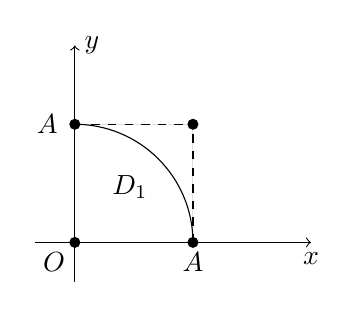
\begin{tikzpicture}
				\coordinate (left) at (-0.5, 0.0);
				\coordinate (right) at (3.0, 0.0);
				\coordinate (top) at (0.0, 2.5);
				\coordinate (bottom) at (0.0, -0.5);
				\coordinate (center) at (0.0, 0.0);
				\draw[->] (left) -- (right);
				\draw[->] (bottom) -- (top);
				\draw (center) node[anchor=north east] {$O$};
				\draw (right) node[anchor=north] {$x$};
				\draw (top) node[anchor=west] {$y$};
				\draw (1.5, 0) arc(0:90:1.5);
				\draw[fill=black, dashed] (0, 1.5) -- (1.5, 1.5);
				\draw[fill=black, dashed] (1.5, 0) -- (1.5, 1.5);
                \draw (-0.35,1.5) node[anchor=center] {$A$};
				\draw (0.7,0.7) node[anchor=center] {$D_1$};
				\draw (1.5, 0) node[anchor=north] {$A$};
				\fill [black] (1.5,1.5) circle (2pt);
				\fill [black] (1.5,0) circle (2pt);
				\fill [black] (0, 1.5) circle (2pt);
				\fill [black] (0, 0) circle (2pt);
			\end{tikzpicture}
		\end{minipage}%
		\begin{minipage}{.5\textwidth}
			\centering
			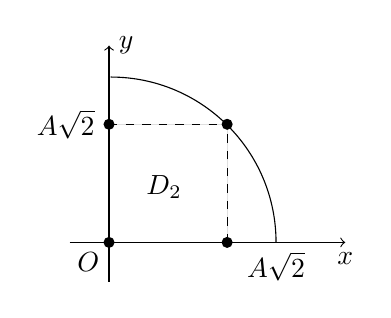
\begin{tikzpicture}
				\coordinate (left) at (-0.5, 0.0);
				\coordinate (right) at (3.0, 0.0);
				\coordinate (top) at (0.0, 2.5);
				\coordinate (bottom) at (0.0, -0.5);
				\coordinate (center) at (0.0, 0.0);
				\draw[->] (left) -- (right);
				\draw[->] (bottom) -- (top);
				\draw (center) node[anchor=north east] {$O$};
				\draw (right) node[anchor=north] {$x$};
				\draw (top) node[anchor=west] {$y$};
				\draw (2.121, 0) arc(0:90:2.1);
				\draw[fill=black, dashed] (0, 1.5) -- (1.5, 1.5);
				\draw[fill=black, dashed] (1.5, 0) -- (1.5, 1.5);
				\draw (0.7,0.7) node[anchor=center] {$D_2$};
				\draw (2.121, 0) node[anchor=north] {$A\sqrt{2}$};
                \draw (-0.55,1.5) node[anchor=center] {$A\sqrt{2}$};
				\fill [black] (1.5,1.5) circle (2pt);
				\fill [black] (1.5,0) circle (2pt);
				\fill [black] (0, 1.5) circle (2pt);
				\fill [black] (0, 0) circle (2pt);
			\end{tikzpicture}
		\end{minipage}
	\end{figure}

	Для $\fix R > 0$, используя полярную замену, вычислим:
	\begin{equation}
		\label{eq:lecture7-29}
		G(R) = \iint\limits_{x^2 + y^2 \leqslant R^2}e^{-(x^2 + y^2)}dxdy.
	\end{equation}
	Имеем:
	\begin{equation*}
		\begin{split}
			&G(R) = \sqcase{x = r \cos \phi, y = r \sin \phi, J = r,
			  \phi \vert_0^{\pi/2}, r\vert_0^R} =
			\iint\limits_{\substack{0\leqslant\phi\leqslant \pi / 2\\
				0 \leqslant r \leqslant R}}r e^{-r^2}dr =
			\int\limits_0^{\pi/2}d\phi \int\limits_0^Rr e^{-r^2}dr = \\
			&=\parenthesis{\sqcase{\phi}_0^{\pi/2}}
			\parenthesis{-\dfrac{1}{2}\sqcase{e^{-r^2}}_0^R} =
			\dfrac{\pi}{4}(1 - e^{-R^2}).
		\end{split}
	\end{equation*}
    \newpage
	Применяя этот результат для $R = A$ и $R = A \sqrt{2}$ и учитывая, что в силу
	\eqref{eq:lecture7-28}, \eqref{eq:lecture7-29} имеем:
	$G(A) \leqslant F(A) \leqslant G(A \sqrt{2})$, для \eqref{eq:lecture7-27}
	получаем:
	\begin{equation*}
		\dfrac{\pi}{4}(1 - e^{-A^2}) \leqslant F(A) \leqslant
		\dfrac{\pi}{4}(1 - e^{-2A^2}).
	\end{equation*}
	Отсюда при $ A \to + \infty $ получаем:
	\begin{equation*}
		\exists F(+\infty) =
		\lim\limits_{A \to +\infty}F(A) = \dfrac{\pi}{4}.
	\end{equation*}

	С другой стороны, вычисляя \eqref{eq:lecture7-27} через повторные интегралы,
	после разбиения переменных, получаем:
	\begin{equation*}
		F(A) = \int\limits_0^Adx\int\limits_0^A e^{-(x^2 + y^2)}dy =
		\int\limits_0^A e^{-x^2}dx \int\limits_0^A e^{-y^2}dy,
	\end{equation*}
	т.е. $F(A)$ - произведение двух одинаковых сомножителей вида
	\eqref{eq:lecture7-25}, в каждом из которых вместо $t$ используются
	соответствующие $x$ и $y$.

	$I^2(A) = F(A) \xrightarrow[A \to +\infty]{} \dfrac{\pi}{4}$. 
    Отсюда	$I_0^2 = \lim\limits_{A \to +\infty}I^2(A) = \dfrac{\pi}{4}$.
    
    Учитывая, что
	в \eqref{eq:lecture7-23} подынтегральная функция неотрицательна, а,
	значит, $I_0 \geqslant 0$, получаем: $I_0 = \sqrt{\dfrac{\pi}{4}} =
	\dfrac{\sqrt{\pi}}{2}$, что даёт \eqref{eq:lecture7-26}.
\end{proof}

\begin{consequence}[обобщение интеграла Эйлера-Пуассона]
	Для $\forall a > 0 \Rightarrow$
	\begin{equation}
		\label{eq:lecture7-30}
		\boxed{\int\limits_0^{+\infty}e^{-ax^2}dx =
		\dfrac{1}{2}\sqrt{\dfrac{\pi}{a}}}
	\end{equation}
\end{consequence}
\begin{proof}
	Достаточно воспользоваться заменой
	\begin{equation*}
		x = \dfrac{t}{\sqrt{a}} \Rightarrow t = x \sqrt{a}\vert_0^{+\infty};
		dx = \dfrac{dt}{\sqrt{a}}.
	\end{equation*}
	Тогда
	\begin{equation*}
		\int\limits_0^{+\infty}e^{-ax^2}dx = \int\limits_0^{+\infty}e^{-a\parenthesis{\frac{t}{\sqrt{a}}}^2}
		\dfrac{dt}{\sqrt{a}} = \dfrac{1}{\sqrt{a}}\int\limits_0^{+\infty}e^{-t^2}dt
		= \dfrac{1}{2}\sqrt{\dfrac{\pi}{a}}
	\end{equation*}
\end{proof}
\begin{examples}
  \item Если $a > 0$ и $b, c \in \R{}$, то
	\begin{equation*}
		\begin{split}
			&\int\limits_{-\infty}^{\infty}e^{-(ax^2 + bx + c)}dx = \int\limits_{-\infty}^{\infty}
			e^{-a(x^2 + \frac{2b}{a}x) - c}dx = \begin{sqcases}x + \frac{b}{a} = 
            t \vert_{-\infty}^{+\infty} 
            \\dx = dt\end{sqcases} =\\
			&=e^{\frac{b^2 - ac}{a}}\int\limits_{-\infty}^{+\infty}e^{-at^2}dt =
			2e^{\frac{b^2 - ac}{a}}\int\limits_{0}^{+\infty}e^{-at^2}dt =
			\sqrt{\dfrac{\pi}{a}}e^{\frac{b^2 - ac}{a}}
		\end{split}
	\end{equation*}
  \item Для $a > 0$ и $b \in \R{}$:
	\begin{equation*}
		\begin{split}
			&\int\limits_{-\infty}^{+\infty}e^{-ax^2}\ch(2bx)dx = \int\limits_{-\infty}^{+\infty}
			e^{-ax^2}\dfrac{e^{2bx} + e^{-2bx}}{2}dx = \dfrac{1}{2}
			\parenthesis{\int\limits_{-\infty}^{+\infty}e^{-(ax^2-2bx)} dx +
			  \int\limits_{-\infty}^{+\infty}e^{-(ax^2+2bx)} dx } =\\
			& = \sqcase{\text{смотри предыдущий пример}} =
			\dfrac{1}{2}\sqrt{\dfrac{\pi}{a}} \parenthesis{e^{b^2/a} + e^{b^2/a}} 
			= \sqrt{\dfrac{\pi}{a}} e^{b^2/a}.
		\end{split}
	\end{equation*}
  \item Для $n \in \mathbb{N}_0$ рассмотрим
	\begin{equation*}
		I_n = \int\limits_0^{+\infty}e^{-x^2}x^{2n}dx,
	\end{equation*}
	имеем
	\begin{equation*}
		I_0 = \int\limits_0^{+\infty}e^{-x^2}dx = \sqrt{\dfrac{\pi}{4}}.
	\end{equation*}
	Далее для $\forall \; n \in \mathbb{N}$, интегрируя по частям, получаем:
	\begin{equation*}
		\begin{split}
			&I_1 = - \dfrac{1}{2}\int\limits_0^{+\infty}x^{2n - 1}d(e^{-x^2}) =
			-\dfrac{1}{2}\sqcase{x^{2n - 1}e^{-x^2}}_0^{+\infty} - \int\limits_0^{+\infty}
			e^{-x^2}d(x^{2n - 1}) =\\
			&=\sqcase{ \;\lim\limits_{x \to +\infty}x^{2n - 1}e^{-x^2} =
			  \lim\limits_{x \to \infty}\dfrac{x^{2n - 1}}{e^{x^2}} = 
              \left[\dfrac{\infty}{\infty}\right] \eqlhopital \ldots = 0 \; } =
			\dfrac{2n - 1}{2}\int\limits_0^{+\infty}e^{-x^2}x^{2n - 2}dx.\\
		\end{split}
	\end{equation*}
	Из полученного рекуррентного соотношения
	\begin{equation*}
		I_n = \dfrac{2n - 1}{2}I_{n - 1}, n \in \mathbb{N},
	\end{equation*}
	последовательно имеем:
	\begin{equation*}
		I_n = \dfrac{2n - 1}{2}\cdot\dfrac{2n - 3}{2}\cdot I_{n - 2}= \ldots =
		\dfrac{1 \cdot 3 \cdot 5 \cdot \ldots \cdot (2n - 1)}{2^n} \cdot
		\dfrac{\sqrt{\pi}}{2} = \dfrac{(2n - 1)!!}{2^{n + 1}}\sqrt{\pi}.
	\end{equation*}
  \item Для $a \geqslant 0\Rightarrow$
	\begin{equation*}
		\begin{split}
			&\int\limits_0^{+\infty}e^{-(x^2 + \frac{a^2}{x^2})}dx =
			\begin{sqcases}
				&x^2 + \frac{a^2}{x^2} = \parenthesis{x - \frac{a}{x}}^2 + 2a;\\
				&t = x - \frac{a}{x};\\
				&x^2 - tx - a = 0 \Leftrightarrow x = \frac{t \pm \sqrt{t^2 + 4a}}{2};\\
				&x \vert_0^{+\infty}\Rightarrow x = \frac{t + \sqrt{t^2 + 4a}}{2},\\
				&t = \parenthesis{x - \frac{a}{x}}\vert_{-\infty}^{+\infty};\\
				&dx = \frac{1}{2}\parenthesis{1 + \frac{t}{\sqrt{t^2 + 4a}}}dt;
			\end{sqcases} = \\
            & = \dfrac{1}{2}\parenthesis{e^{2a}
			  \underbrace{\int\limits_{-\infty}^{+\infty}e^{-t^2}dt}_{\text{чётная}}
			  + e^{2a}
			  \underbrace{\int\limits_{-\infty}^{+\infty}\dfrac{te^{-t^2}}
				{\sqrt{t^2 + 4a}}dt}_{\text{нечётная}}} 
			=\dfrac{1}{2}e^{2a}\parenthesis{2\int\limits_0^{+\infty}e^{-t^2}dt} =
			e^{2a}\sqrt{\dfrac{\pi}{4}}.
		\end{split}
	\end{equation*}
\end{examples}

$  $\newpage

$  $
